\chapter{Implementierung}
test



\section{Softwaredokumentation}

\subsection{Aufnahme von Tastatureingaben}
\subsubsection{readKeys()}
\subsubsection{writeSd()}
\subsubsection{reader()}
\begin{figure}
  \centering
  %\includegraphics[angle=90,width=1\textwidth]{images/diagram_reader.png}
  \caption{Aktivitätsdiagramm für die Methode reader()}
  \label{diagram_reader}
\end{figure}

\subsection{Wiedergabe von Tastatureingaben mittels SD-Karte}
\subsubsection{readSd()}
\subsubsection{writeKeys()}
\subsubsection{writer()}
\begin{figure}
  \centering
  %\includegraphics[angle=90,width=1\textwidth]{images/diagram_writer.png}
  \caption{Aktivitätsdiagramm für die Methode writer()}
  \label{diagram_writer}
\end{figure}

\subsection{Wiedergabe von Tastatureingaben über Ethernet}
\subsubsection{sendWebsite()}
\subsubsection{writeKeys()}
\subsubsection{sender()}
\begin{figure}
  \centering
  %\includegraphics[angle=90,width=1\textwidth]{images/diagram_sender.png}
  \caption{Aktivitätsdiagramm für die Methode sender()}
  \label{diagram_sender}
\end{figure}

\subsection{Gesamter Programmablauf}



\section{Aufbau der Elektronik}
Verwendete Kabel \cite{ps2male} \cite{ps2female}, Arduino Mega und Ethernet \cite{arduino} und PS/2-Tastatur.
\begin{figure}
  \centering
  \begin{minipage}{0.45\textwidth}
    \centering
    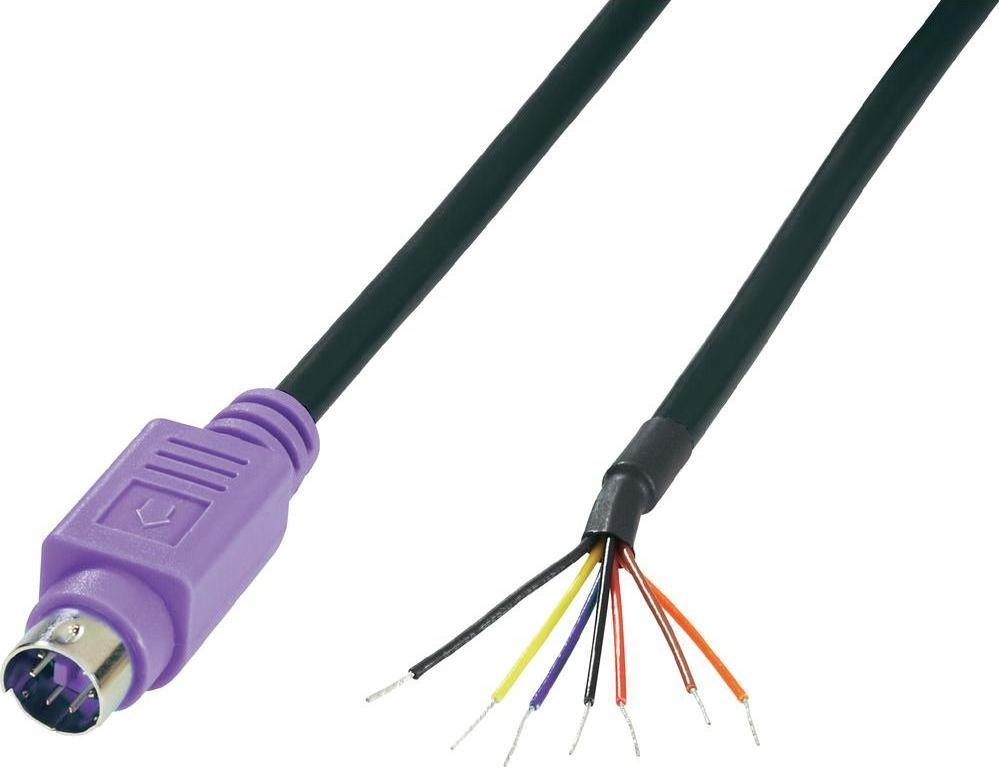
\includegraphics[width=1\textwidth]{images/ps2_male.jpg}
    \caption{PS/2 Male}
    \label{ps2_male}
  \end{minipage}
  \begin{minipage}{0.45\textwidth}
    \centering
    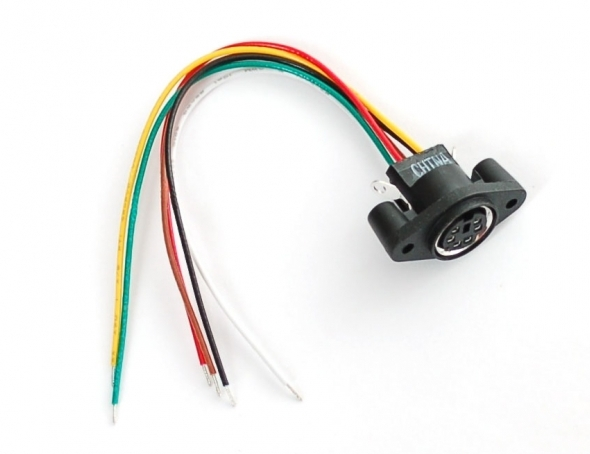
\includegraphics[width=1\textwidth]{images/ps2_female.jpg}
    \caption{PS/2 Female}
    \label{ps2_female}
  \end{minipage}
\end{figure}

\begin{figure}
  \centering
  %\includegraphics[width=0.8\textwidth]{images/hall_effect_sensor.jpg}
  \caption{Schema des Aufbaus fritzing}
  \label{fritzing}
\end{figure}

\begin{figure}
  \centering
  %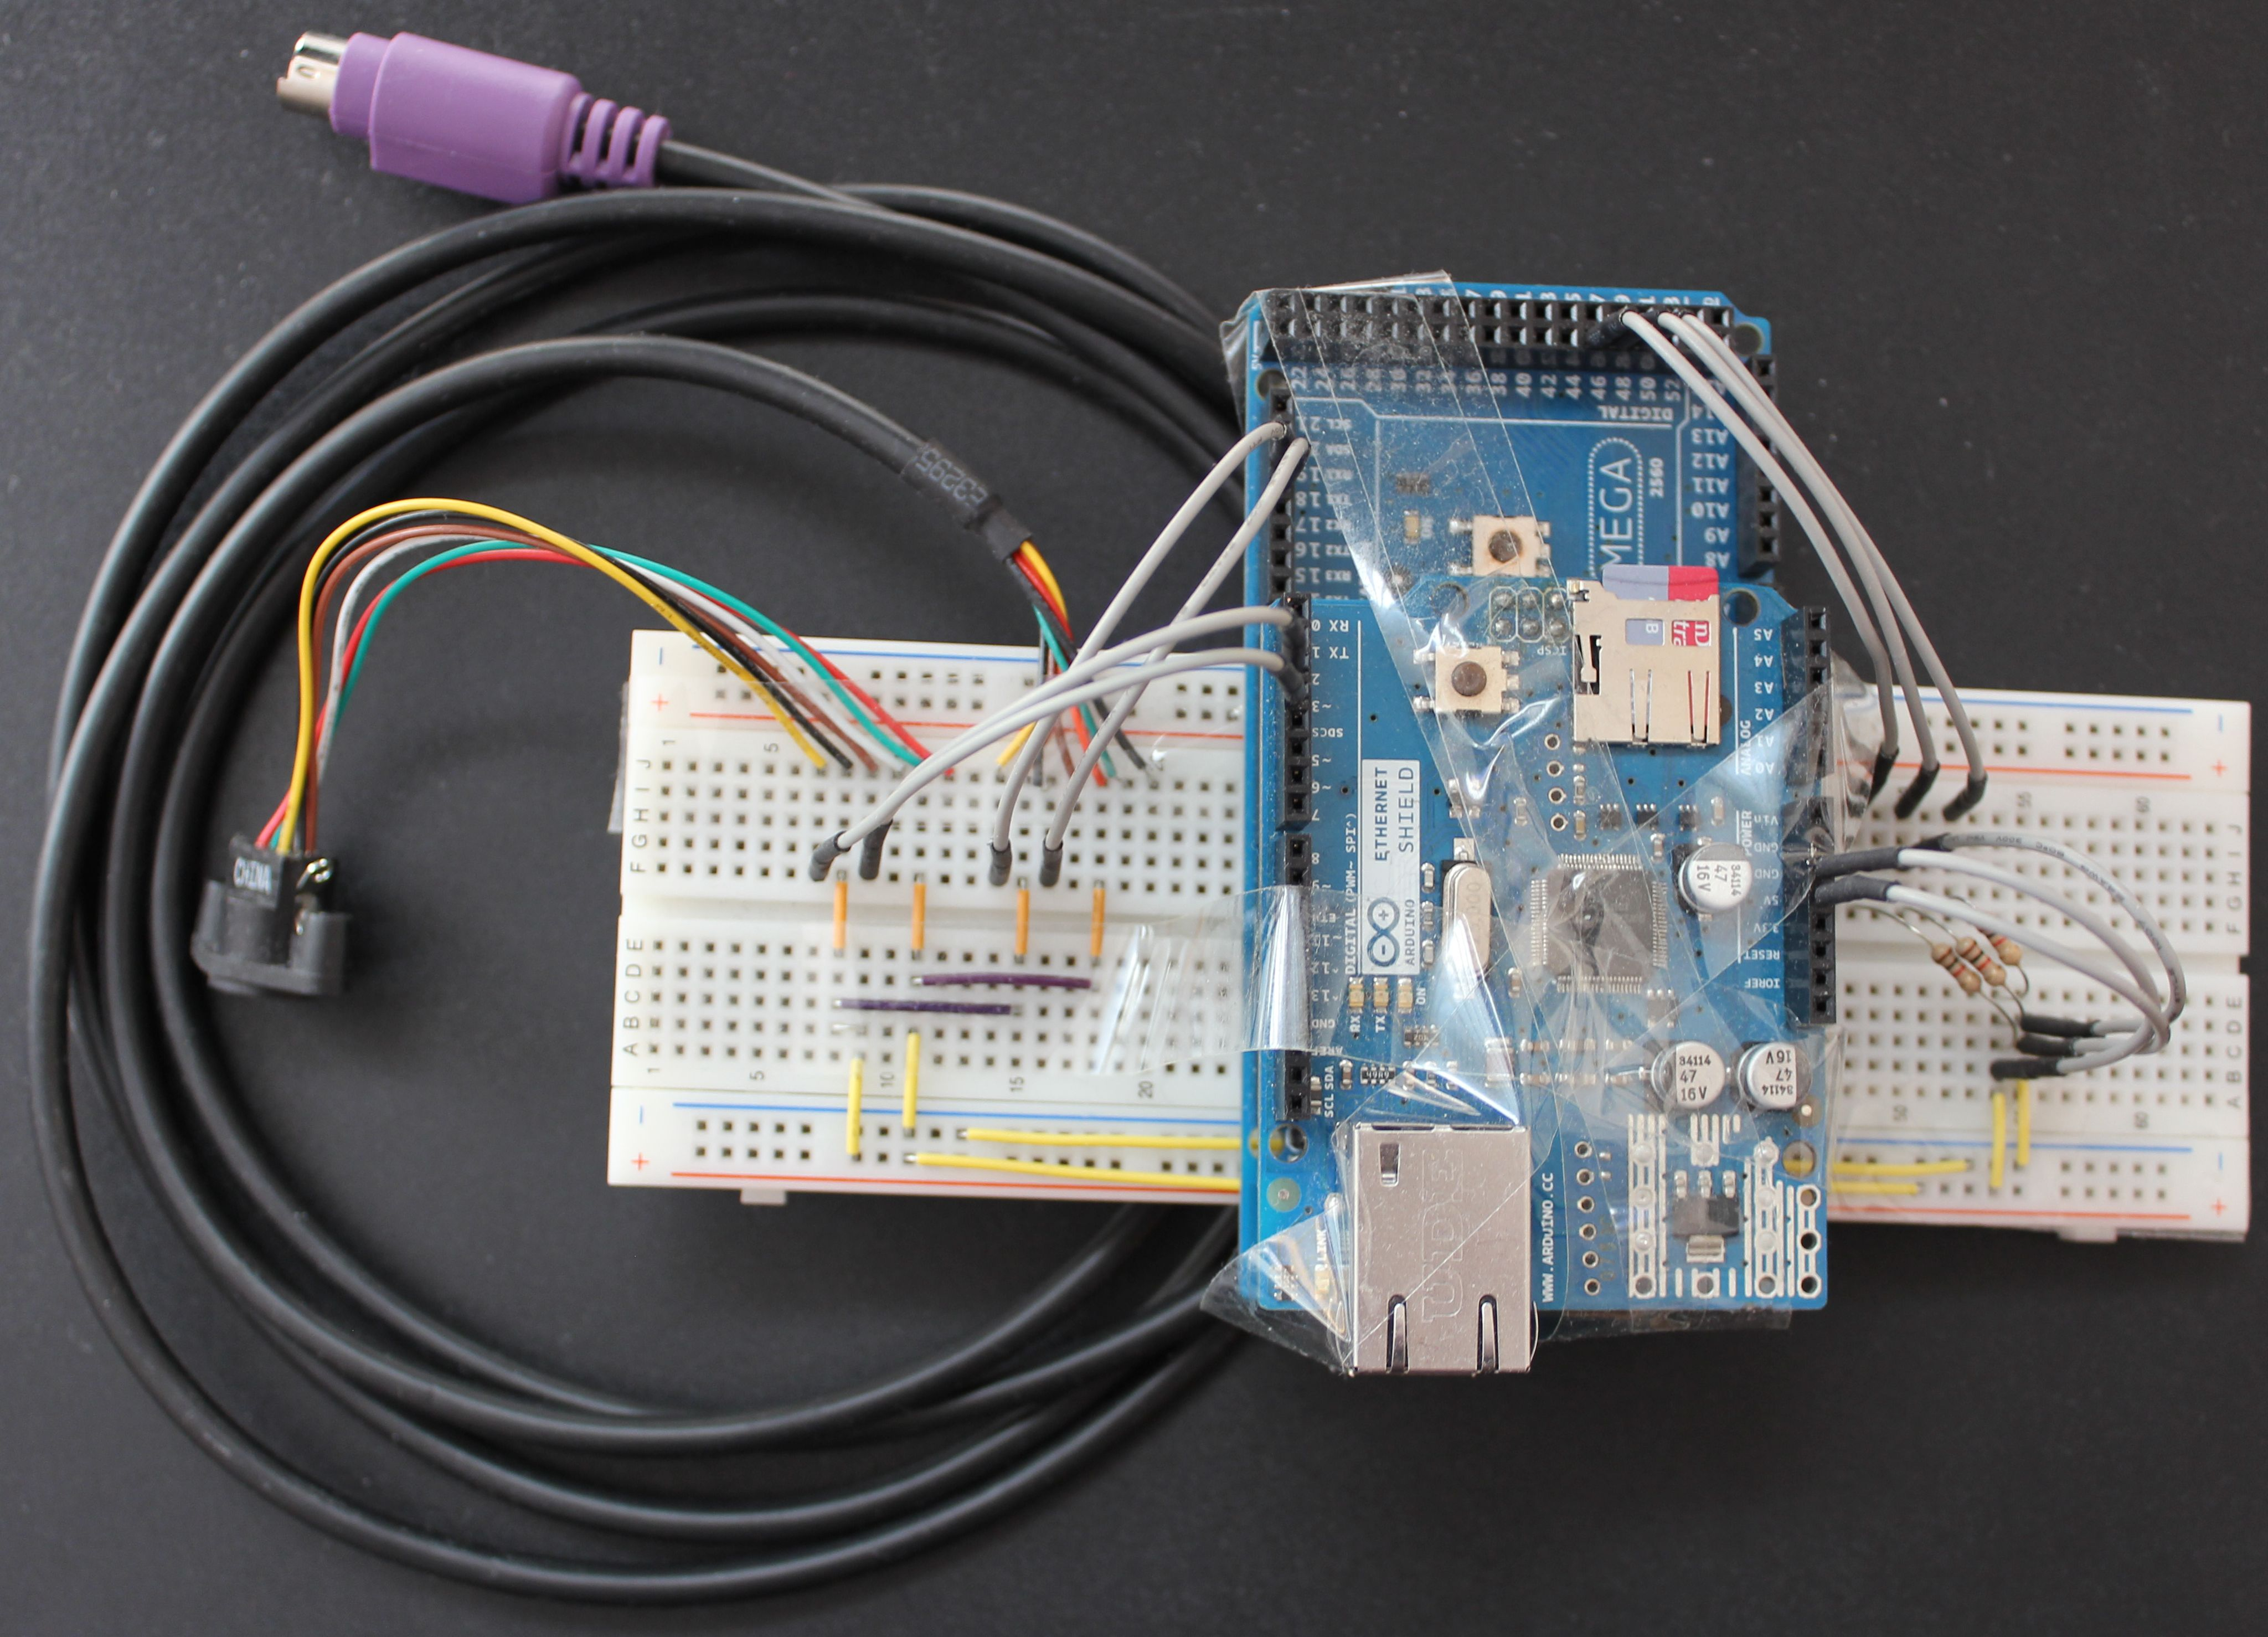
\includegraphics[width=0.8\textwidth]{images/foto1.jpg}
  \caption{Foto des Arduino Ethernet Shields und des Mega 2560 Boards}
  \label{foto1}
\end{figure}